\documentclass[11pt]{extarticle}
\usepackage[a4paper, total={6in, 8.5in}, top=1in, bottom=1in, left=1in, right=1in]{geometry}

\usepackage{mathtools}
\usepackage{graphicx}
\usepackage{amssymb}
\usepackage{amsmath}
\usepackage{pythonhighlight}
\usepackage{pdfpages}
\usepackage[T1]{fontenc}
\usepackage[utf8]{inputenc}
\usepackage{fancyhdr}
\usepackage{pythonhighlight}
\usepackage{changepage}
\usepackage{slashbox}
\usepackage{floatrow}
\usepackage{listings}
\usepackage[hidelinks]{hyperref}
\usepackage{fontawesome}
\usepackage{caption}
\usepackage{subcaption}
\usepackage{pdfpages}
\usepackage{color} %red, green, blue, yellow, cyan, magenta, black, white
\definecolor{mygreen}{RGB}{28,172,0} % color values Red, Green, Blue
\definecolor{mylilas}{RGB}{170,55,241}


\usepackage[breakable]{tcolorbox}
\usepackage{parskip} % Stop auto-indenting (to mimic markdown behaviour)

\usepackage{iftex}
\ifPDFTeX
    \usepackage[T1]{fontenc}
    \usepackage{mathpazo}
\else
    \usepackage{fontspec}
\fi

% Basic figure setup, for now with no caption control since it's done
% automatically by Pandoc (which extracts ![](path) syntax from Markdown).
\usepackage{graphicx}
% Maintain compatibility with old templates. Remove in nbconvert 6.0
\let\Oldincludegraphics\includegraphics
% Ensure that by default, figures have no caption (until we provide a
% proper Figure object with a Caption API and a way to capture that
% in the conversion process - todo).
\usepackage{caption}
\DeclareCaptionFormat{nocaption}{}
\captionsetup{format=nocaption,aboveskip=0pt,belowskip=0pt}

\usepackage[Export]{adjustbox} % Used to constrain images to a maximum size
\adjustboxset{max size={0.9\linewidth}{0.9\paperheight}}
\usepackage{float}
\floatplacement{figure}{H} % forces figures to be placed at the correct location
\usepackage{xcolor} % Allow colors to be defined
\usepackage{enumerate} % Needed for markdown enumerations to work
\usepackage{geometry} % Used to adjust the document margins
\usepackage{amsmath} % Equations
\usepackage{amssymb} % Equations
\usepackage{textcomp} % defines textquotesingle
% Hack from http://tex.stackexchange.com/a/47451/13684:
\AtBeginDocument{%
    \def\PYZsq{\textquotesingle}% Upright quotes in Pygmentized code
}
\usepackage{upquote} % Upright quotes for verbatim code
\usepackage{eurosym} % defines \euro
\usepackage[mathletters]{ucs} % Extended unicode (utf-8) support
\usepackage{fancyvrb} % verbatim replacement that allows latex
\usepackage{grffile} % extends the file name processing of package graphics 
                        % to support a larger range
\makeatletter % fix for grffile with XeLaTeX
\def\Gread@@xetex#1{%
    \IfFileExists{"\Gin@base".bb}%
    {\Gread@eps{\Gin@base.bb}}%
    {\Gread@@xetex@aux#1}%
}
\makeatother

% The hyperref package gives us a pdf with properly built
% internal navigation ('pdf bookmarks' for the table of contents,
% internal cross-reference links, web links for URLs, etc.)
\usepackage{hyperref}
% The default LaTeX title has an obnoxious amount of whitespace. By default,
% titling removes some of it. It also provides customization options.
\usepackage{titling}
\usepackage{longtable} % longtable support required by pandoc >1.10
\usepackage{booktabs}  % table support for pandoc > 1.12.2
\usepackage[inline]{enumitem} % IRkernel/repr support (it uses the enumerate* environment)
\usepackage[normalem]{ulem} % ulem is needed to support strikethroughs (\sout)
                            % normalem makes italics be italics, not underlines
\usepackage{mathrsfs}



% Colors for the hyperref package
\definecolor{urlcolor}{rgb}{0,.145,.698}
\definecolor{linkcolor}{rgb}{0,0,0}
\definecolor{citecolor}{rgb}{.12,.54,.11}

% ANSI colors
\definecolor{ansi-black}{HTML}{3E424D}
\definecolor{ansi-black-intense}{HTML}{282C36}
\definecolor{ansi-red}{HTML}{E75C58}
\definecolor{ansi-red-intense}{HTML}{B22B31}
\definecolor{ansi-green}{HTML}{00A250}
\definecolor{ansi-green-intense}{HTML}{007427}
\definecolor{ansi-yellow}{HTML}{DDB62B}
\definecolor{ansi-yellow-intense}{HTML}{B27D12}
\definecolor{ansi-blue}{HTML}{208FFB}
\definecolor{ansi-blue-intense}{HTML}{0065CA}
\definecolor{ansi-magenta}{HTML}{D160C4}
\definecolor{ansi-magenta-intense}{HTML}{A03196}
\definecolor{ansi-cyan}{HTML}{60C6C8}
\definecolor{ansi-cyan-intense}{HTML}{258F8F}
\definecolor{ansi-white}{HTML}{C5C1B4}
\definecolor{ansi-white-intense}{HTML}{A1A6B2}
\definecolor{ansi-default-inverse-fg}{HTML}{FFFFFF}
\definecolor{ansi-default-inverse-bg}{HTML}{000000}

% commands and environments needed by pandoc snippets
% extracted from the output of `pandoc -s`
\providecommand{\tightlist}{%
    \setlength{\itemsep}{0pt}\setlength{\parskip}{0pt}}
\DefineVerbatimEnvironment{Highlighting}{Verbatim}{commandchars=\\\{\}}
% Add ',fontsize=\small' for more characters per line
\newenvironment{Shaded}{}{}
\newcommand{\KeywordTok}[1]{\textcolor[rgb]{0.00,0.44,0.13}{\textbf{{#1}}}}
\newcommand{\DataTypeTok}[1]{\textcolor[rgb]{0.56,0.13,0.00}{{#1}}}
\newcommand{\DecValTok}[1]{\textcolor[rgb]{0.25,0.63,0.44}{{#1}}}
\newcommand{\BaseNTok}[1]{\textcolor[rgb]{0.25,0.63,0.44}{{#1}}}
\newcommand{\FloatTok}[1]{\textcolor[rgb]{0.25,0.63,0.44}{{#1}}}
\newcommand{\CharTok}[1]{\textcolor[rgb]{0.25,0.44,0.63}{{#1}}}
\newcommand{\StringTok}[1]{\textcolor[rgb]{0.25,0.44,0.63}{{#1}}}
\newcommand{\CommentTok}[1]{\textcolor[rgb]{0.38,0.63,0.69}{\textit{{#1}}}}
\newcommand{\OtherTok}[1]{\textcolor[rgb]{0.00,0.44,0.13}{{#1}}}
\newcommand{\AlertTok}[1]{\textcolor[rgb]{1.00,0.00,0.00}{\textbf{{#1}}}}
\newcommand{\FunctionTok}[1]{\textcolor[rgb]{0.02,0.16,0.49}{{#1}}}
\newcommand{\RegionMarkerTok}[1]{{#1}}
\newcommand{\ErrorTok}[1]{\textcolor[rgb]{1.00,0.00,0.00}{\textbf{{#1}}}}
\newcommand{\NormalTok}[1]{{#1}}

% Additional commands for more recent versions of Pandoc
\newcommand{\ConstantTok}[1]{\textcolor[rgb]{0.53,0.00,0.00}{{#1}}}
\newcommand{\SpecialCharTok}[1]{\textcolor[rgb]{0.25,0.44,0.63}{{#1}}}
\newcommand{\VerbatimStringTok}[1]{\textcolor[rgb]{0.25,0.44,0.63}{{#1}}}
\newcommand{\SpecialStringTok}[1]{\textcolor[rgb]{0.73,0.40,0.53}{{#1}}}
\newcommand{\ImportTok}[1]{{#1}}
\newcommand{\DocumentationTok}[1]{\textcolor[rgb]{0.73,0.13,0.13}{\textit{{#1}}}}
\newcommand{\AnnotationTok}[1]{\textcolor[rgb]{0.38,0.63,0.69}{\textbf{\textit{{#1}}}}}
\newcommand{\CommentVarTok}[1]{\textcolor[rgb]{0.38,0.63,0.69}{\textbf{\textit{{#1}}}}}
\newcommand{\VariableTok}[1]{\textcolor[rgb]{0.10,0.09,0.49}{{#1}}}
\newcommand{\ControlFlowTok}[1]{\textcolor[rgb]{0.00,0.44,0.13}{\textbf{{#1}}}}
\newcommand{\OperatorTok}[1]{\textcolor[rgb]{0.40,0.40,0.40}{{#1}}}
\newcommand{\BuiltInTok}[1]{{#1}}
\newcommand{\ExtensionTok}[1]{{#1}}
\newcommand{\PreprocessorTok}[1]{\textcolor[rgb]{0.74,0.48,0.00}{{#1}}}
\newcommand{\AttributeTok}[1]{\textcolor[rgb]{0.49,0.56,0.16}{{#1}}}
\newcommand{\InformationTok}[1]{\textcolor[rgb]{0.38,0.63,0.69}{\textbf{\textit{{#1}}}}}
\newcommand{\WarningTok}[1]{\textcolor[rgb]{0.38,0.63,0.69}{\textbf{\textit{{#1}}}}}


% Define a nice break command that doesn't care if a line doesn't already
% exist.
\def\br{\hspace*{\fill} \\* }
% Math Jax compatibility definitions
\def\gt{>}
\def\lt{<}
\let\Oldtex\TeX
\let\Oldlatex\LaTeX
\renewcommand{\TeX}{\textrm{\Oldtex}}
\renewcommand{\LaTeX}{\textrm{\Oldlatex}}
% Document parameters
% Document title
\title{APPENDIX}





% Pygments definitions
\makeatletter
\def\PY@reset{\let\PY@it=\relax \let\PY@bf=\relax%
\let\PY@ul=\relax \let\PY@tc=\relax%
\let\PY@bc=\relax \let\PY@ff=\relax}
\def\PY@tok#1{\csname PY@tok@#1\endcsname}
\def\PY@toks#1+{\ifx\relax#1\empty\else%
\PY@tok{#1}\expandafter\PY@toks\fi}
\def\PY@do#1{\PY@bc{\PY@tc{\PY@ul{%
\PY@it{\PY@bf{\PY@ff{#1}}}}}}}
\def\PY#1#2{\PY@reset\PY@toks#1+\relax+\PY@do{#2}}

\expandafter\def\csname PY@tok@w\endcsname{\def\PY@tc##1{\textcolor[rgb]{0.73,0.73,0.73}{##1}}}
\expandafter\def\csname PY@tok@c\endcsname{\let\PY@it=\textit\def\PY@tc##1{\textcolor[rgb]{0.25,0.50,0.50}{##1}}}
\expandafter\def\csname PY@tok@cp\endcsname{\def\PY@tc##1{\textcolor[rgb]{0.74,0.48,0.00}{##1}}}
\expandafter\def\csname PY@tok@k\endcsname{\let\PY@bf=\textbf\def\PY@tc##1{\textcolor[rgb]{0.00,0.50,0.00}{##1}}}
\expandafter\def\csname PY@tok@kp\endcsname{\def\PY@tc##1{\textcolor[rgb]{0.00,0.50,0.00}{##1}}}
\expandafter\def\csname PY@tok@kt\endcsname{\def\PY@tc##1{\textcolor[rgb]{0.69,0.00,0.25}{##1}}}
\expandafter\def\csname PY@tok@o\endcsname{\def\PY@tc##1{\textcolor[rgb]{0.40,0.40,0.40}{##1}}}
\expandafter\def\csname PY@tok@ow\endcsname{\let\PY@bf=\textbf\def\PY@tc##1{\textcolor[rgb]{0.67,0.13,1.00}{##1}}}
\expandafter\def\csname PY@tok@nb\endcsname{\def\PY@tc##1{\textcolor[rgb]{0.00,0.50,0.00}{##1}}}
\expandafter\def\csname PY@tok@nf\endcsname{\def\PY@tc##1{\textcolor[rgb]{0.00,0.00,1.00}{##1}}}
\expandafter\def\csname PY@tok@nc\endcsname{\let\PY@bf=\textbf\def\PY@tc##1{\textcolor[rgb]{0.00,0.00,1.00}{##1}}}
\expandafter\def\csname PY@tok@nn\endcsname{\let\PY@bf=\textbf\def\PY@tc##1{\textcolor[rgb]{0.00,0.00,1.00}{##1}}}
\expandafter\def\csname PY@tok@ne\endcsname{\let\PY@bf=\textbf\def\PY@tc##1{\textcolor[rgb]{0.82,0.25,0.23}{##1}}}
\expandafter\def\csname PY@tok@nv\endcsname{\def\PY@tc##1{\textcolor[rgb]{0.10,0.09,0.49}{##1}}}
\expandafter\def\csname PY@tok@no\endcsname{\def\PY@tc##1{\textcolor[rgb]{0.53,0.00,0.00}{##1}}}
\expandafter\def\csname PY@tok@nl\endcsname{\def\PY@tc##1{\textcolor[rgb]{0.63,0.63,0.00}{##1}}}
\expandafter\def\csname PY@tok@ni\endcsname{\let\PY@bf=\textbf\def\PY@tc##1{\textcolor[rgb]{0.60,0.60,0.60}{##1}}}
\expandafter\def\csname PY@tok@na\endcsname{\def\PY@tc##1{\textcolor[rgb]{0.49,0.56,0.16}{##1}}}
\expandafter\def\csname PY@tok@nt\endcsname{\let\PY@bf=\textbf\def\PY@tc##1{\textcolor[rgb]{0.00,0.50,0.00}{##1}}}
\expandafter\def\csname PY@tok@nd\endcsname{\def\PY@tc##1{\textcolor[rgb]{0.67,0.13,1.00}{##1}}}
\expandafter\def\csname PY@tok@s\endcsname{\def\PY@tc##1{\textcolor[rgb]{0.73,0.13,0.13}{##1}}}
\expandafter\def\csname PY@tok@sd\endcsname{\let\PY@it=\textit\def\PY@tc##1{\textcolor[rgb]{0.73,0.13,0.13}{##1}}}
\expandafter\def\csname PY@tok@si\endcsname{\let\PY@bf=\textbf\def\PY@tc##1{\textcolor[rgb]{0.73,0.40,0.53}{##1}}}
\expandafter\def\csname PY@tok@se\endcsname{\let\PY@bf=\textbf\def\PY@tc##1{\textcolor[rgb]{0.73,0.40,0.13}{##1}}}
\expandafter\def\csname PY@tok@sr\endcsname{\def\PY@tc##1{\textcolor[rgb]{0.73,0.40,0.53}{##1}}}
\expandafter\def\csname PY@tok@ss\endcsname{\def\PY@tc##1{\textcolor[rgb]{0.10,0.09,0.49}{##1}}}
\expandafter\def\csname PY@tok@sx\endcsname{\def\PY@tc##1{\textcolor[rgb]{0.00,0.50,0.00}{##1}}}
\expandafter\def\csname PY@tok@m\endcsname{\def\PY@tc##1{\textcolor[rgb]{0.40,0.40,0.40}{##1}}}
\expandafter\def\csname PY@tok@gh\endcsname{\let\PY@bf=\textbf\def\PY@tc##1{\textcolor[rgb]{0.00,0.00,0.50}{##1}}}
\expandafter\def\csname PY@tok@gu\endcsname{\let\PY@bf=\textbf\def\PY@tc##1{\textcolor[rgb]{0.50,0.00,0.50}{##1}}}
\expandafter\def\csname PY@tok@gd\endcsname{\def\PY@tc##1{\textcolor[rgb]{0.63,0.00,0.00}{##1}}}
\expandafter\def\csname PY@tok@gi\endcsname{\def\PY@tc##1{\textcolor[rgb]{0.00,0.63,0.00}{##1}}}
\expandafter\def\csname PY@tok@gr\endcsname{\def\PY@tc##1{\textcolor[rgb]{1.00,0.00,0.00}{##1}}}
\expandafter\def\csname PY@tok@ge\endcsname{\let\PY@it=\textit}
\expandafter\def\csname PY@tok@gs\endcsname{\let\PY@bf=\textbf}
\expandafter\def\csname PY@tok@gp\endcsname{\let\PY@bf=\textbf\def\PY@tc##1{\textcolor[rgb]{0.00,0.00,0.50}{##1}}}
\expandafter\def\csname PY@tok@go\endcsname{\def\PY@tc##1{\textcolor[rgb]{0.53,0.53,0.53}{##1}}}
\expandafter\def\csname PY@tok@gt\endcsname{\def\PY@tc##1{\textcolor[rgb]{0.00,0.27,0.87}{##1}}}
\expandafter\def\csname PY@tok@err\endcsname{\def\PY@bc##1{\setlength{\fboxsep}{0pt}\fcolorbox[rgb]{1.00,0.00,0.00}{1,1,1}{\strut ##1}}}
\expandafter\def\csname PY@tok@kc\endcsname{\let\PY@bf=\textbf\def\PY@tc##1{\textcolor[rgb]{0.00,0.50,0.00}{##1}}}
\expandafter\def\csname PY@tok@kd\endcsname{\let\PY@bf=\textbf\def\PY@tc##1{\textcolor[rgb]{0.00,0.50,0.00}{##1}}}
\expandafter\def\csname PY@tok@kn\endcsname{\let\PY@bf=\textbf\def\PY@tc##1{\textcolor[rgb]{0.00,0.50,0.00}{##1}}}
\expandafter\def\csname PY@tok@kr\endcsname{\let\PY@bf=\textbf\def\PY@tc##1{\textcolor[rgb]{0.00,0.50,0.00}{##1}}}
\expandafter\def\csname PY@tok@bp\endcsname{\def\PY@tc##1{\textcolor[rgb]{0.00,0.50,0.00}{##1}}}
\expandafter\def\csname PY@tok@fm\endcsname{\def\PY@tc##1{\textcolor[rgb]{0.00,0.00,1.00}{##1}}}
\expandafter\def\csname PY@tok@vc\endcsname{\def\PY@tc##1{\textcolor[rgb]{0.10,0.09,0.49}{##1}}}
\expandafter\def\csname PY@tok@vg\endcsname{\def\PY@tc##1{\textcolor[rgb]{0.10,0.09,0.49}{##1}}}
\expandafter\def\csname PY@tok@vi\endcsname{\def\PY@tc##1{\textcolor[rgb]{0.10,0.09,0.49}{##1}}}
\expandafter\def\csname PY@tok@vm\endcsname{\def\PY@tc##1{\textcolor[rgb]{0.10,0.09,0.49}{##1}}}
\expandafter\def\csname PY@tok@sa\endcsname{\def\PY@tc##1{\textcolor[rgb]{0.73,0.13,0.13}{##1}}}
\expandafter\def\csname PY@tok@sb\endcsname{\def\PY@tc##1{\textcolor[rgb]{0.73,0.13,0.13}{##1}}}
\expandafter\def\csname PY@tok@sc\endcsname{\def\PY@tc##1{\textcolor[rgb]{0.73,0.13,0.13}{##1}}}
\expandafter\def\csname PY@tok@dl\endcsname{\def\PY@tc##1{\textcolor[rgb]{0.73,0.13,0.13}{##1}}}
\expandafter\def\csname PY@tok@s2\endcsname{\def\PY@tc##1{\textcolor[rgb]{0.73,0.13,0.13}{##1}}}
\expandafter\def\csname PY@tok@sh\endcsname{\def\PY@tc##1{\textcolor[rgb]{0.73,0.13,0.13}{##1}}}
\expandafter\def\csname PY@tok@s1\endcsname{\def\PY@tc##1{\textcolor[rgb]{0.73,0.13,0.13}{##1}}}
\expandafter\def\csname PY@tok@mb\endcsname{\def\PY@tc##1{\textcolor[rgb]{0.40,0.40,0.40}{##1}}}
\expandafter\def\csname PY@tok@mf\endcsname{\def\PY@tc##1{\textcolor[rgb]{0.40,0.40,0.40}{##1}}}
\expandafter\def\csname PY@tok@mh\endcsname{\def\PY@tc##1{\textcolor[rgb]{0.40,0.40,0.40}{##1}}}
\expandafter\def\csname PY@tok@mi\endcsname{\def\PY@tc##1{\textcolor[rgb]{0.40,0.40,0.40}{##1}}}
\expandafter\def\csname PY@tok@il\endcsname{\def\PY@tc##1{\textcolor[rgb]{0.40,0.40,0.40}{##1}}}
\expandafter\def\csname PY@tok@mo\endcsname{\def\PY@tc##1{\textcolor[rgb]{0.40,0.40,0.40}{##1}}}
\expandafter\def\csname PY@tok@ch\endcsname{\let\PY@it=\textit\def\PY@tc##1{\textcolor[rgb]{0.25,0.50,0.50}{##1}}}
\expandafter\def\csname PY@tok@cm\endcsname{\let\PY@it=\textit\def\PY@tc##1{\textcolor[rgb]{0.25,0.50,0.50}{##1}}}
\expandafter\def\csname PY@tok@cpf\endcsname{\let\PY@it=\textit\def\PY@tc##1{\textcolor[rgb]{0.25,0.50,0.50}{##1}}}
\expandafter\def\csname PY@tok@c1\endcsname{\let\PY@it=\textit\def\PY@tc##1{\textcolor[rgb]{0.25,0.50,0.50}{##1}}}
\expandafter\def\csname PY@tok@cs\endcsname{\let\PY@it=\textit\def\PY@tc##1{\textcolor[rgb]{0.25,0.50,0.50}{##1}}}

\def\PYZbs{\char`\\}
\def\PYZus{\char`\_}
\def\PYZob{\char`\{}
\def\PYZcb{\char`\}}
\def\PYZca{\char`\^}
\def\PYZam{\char`\&}
\def\PYZlt{\char`\<}
\def\PYZgt{\char`\>}
\def\PYZsh{\char`\#}
\def\PYZpc{\char`\%}
\def\PYZdl{\char`\$}
\def\PYZhy{\char`\-}
\def\PYZsq{\char`\'}
\def\PYZdq{\char`\"}
\def\PYZti{\char`\~}
% for compatibility with earlier versions
\def\PYZat{@}
\def\PYZlb{[}
\def\PYZrb{]}
\makeatother


% For linebreaks inside Verbatim environment from package fancyvrb. 
\makeatletter
    \newbox\Wrappedcontinuationbox 
    \newbox\Wrappedvisiblespacebox 
    \newcommand*\Wrappedvisiblespace {\textcolor{red}{\textvisiblespace}} 
    \newcommand*\Wrappedcontinuationsymbol {\textcolor{red}{\llap{\tiny$\m@th\hookrightarrow$}}} 
    \newcommand*\Wrappedcontinuationindent {3ex } 
    \newcommand*\Wrappedafterbreak {\kern\Wrappedcontinuationindent\copy\Wrappedcontinuationbox} 
    % Take advantage of the already applied Pygments mark-up to insert 
    % potential linebreaks for TeX processing. 
    %        {, <, #, %, $, ' and ": go to next line. 
    %        _, }, ^, &, >, - and ~: stay at end of broken line. 
    % Use of \textquotesingle for straight quote. 
    \newcommand*\Wrappedbreaksatspecials {% 
        \def\PYGZus{\discretionary{\char`\_}{\Wrappedafterbreak}{\char`\_}}% 
        \def\PYGZob{\discretionary{}{\Wrappedafterbreak\char`\{}{\char`\{}}% 
        \def\PYGZcb{\discretionary{\char`\}}{\Wrappedafterbreak}{\char`\}}}% 
        \def\PYGZca{\discretionary{\char`\^}{\Wrappedafterbreak}{\char`\^}}% 
        \def\PYGZam{\discretionary{\char`\&}{\Wrappedafterbreak}{\char`\&}}% 
        \def\PYGZlt{\discretionary{}{\Wrappedafterbreak\char`\<}{\char`\<}}% 
        \def\PYGZgt{\discretionary{\char`\>}{\Wrappedafterbreak}{\char`\>}}% 
        \def\PYGZsh{\discretionary{}{\Wrappedafterbreak\char`\#}{\char`\#}}% 
        \def\PYGZpc{\discretionary{}{\Wrappedafterbreak\char`\%}{\char`\%}}% 
        \def\PYGZdl{\discretionary{}{\Wrappedafterbreak\char`\$}{\char`\$}}% 
        \def\PYGZhy{\discretionary{\char`\-}{\Wrappedafterbreak}{\char`\-}}% 
        \def\PYGZsq{\discretionary{}{\Wrappedafterbreak\textquotesingle}{\textquotesingle}}% 
        \def\PYGZdq{\discretionary{}{\Wrappedafterbreak\char`\"}{\char`\"}}% 
        \def\PYGZti{\discretionary{\char`\~}{\Wrappedafterbreak}{\char`\~}}% 
    } 
    % Some characters . , ; ? ! / are not pygmentized. 
    % This macro makes them "active" and they will insert potential linebreaks 
    \newcommand*\Wrappedbreaksatpunct {% 
        \lccode`\~`\.\lowercase{\def~}{\discretionary{\hbox{\char`\.}}{\Wrappedafterbreak}{\hbox{\char`\.}}}% 
        \lccode`\~`\,\lowercase{\def~}{\discretionary{\hbox{\char`\,}}{\Wrappedafterbreak}{\hbox{\char`\,}}}% 
        \lccode`\~`\;\lowercase{\def~}{\discretionary{\hbox{\char`\;}}{\Wrappedafterbreak}{\hbox{\char`\;}}}% 
        \lccode`\~`\:\lowercase{\def~}{\discretionary{\hbox{\char`\:}}{\Wrappedafterbreak}{\hbox{\char`\:}}}% 
        \lccode`\~`\?\lowercase{\def~}{\discretionary{\hbox{\char`\?}}{\Wrappedafterbreak}{\hbox{\char`\?}}}% 
        \lccode`\~`\!\lowercase{\def~}{\discretionary{\hbox{\char`\!}}{\Wrappedafterbreak}{\hbox{\char`\!}}}% 
        \lccode`\~`\/\lowercase{\def~}{\discretionary{\hbox{\char`\/}}{\Wrappedafterbreak}{\hbox{\char`\/}}}% 
        \catcode`\.\active
        \catcode`\,\active 
        \catcode`\;\active
        \catcode`\:\active
        \catcode`\?\active
        \catcode`\!\active
        \catcode`\/\active 
        \lccode`\~`\~ 	
    }
\makeatother

\let\OriginalVerbatim=\Verbatim
\makeatletter
\renewcommand{\Verbatim}[1][1]{%
    %\parskip\z@skip
    \sbox\Wrappedcontinuationbox {\Wrappedcontinuationsymbol}%
    \sbox\Wrappedvisiblespacebox {\FV@SetupFont\Wrappedvisiblespace}%
    \def\FancyVerbFormatLine ##1{\hsize\linewidth
        \vtop{\raggedright\hyphenpenalty\z@\exhyphenpenalty\z@
            \doublehyphendemerits\z@\finalhyphendemerits\z@
            \strut ##1\strut}%
    }%
    % If the linebreak is at a space, the latter will be displayed as visible
    % space at end of first line, and a continuation symbol starts next line.
    % Stretch/shrink are however usually zero for typewriter font.
    \def\FV@Space {%
        \nobreak\hskip\z@ plus\fontdimen3\font minus\fontdimen4\font
        \discretionary{\copy\Wrappedvisiblespacebox}{\Wrappedafterbreak}
        {\kern\fontdimen2\font}%
    }%
    
    % Allow breaks at special characters using \PYG... macros.
    \Wrappedbreaksatspecials
    % Breaks at punctuation characters . , ; ? ! and / need catcode=\active 	
    \OriginalVerbatim[#1,codes*=\Wrappedbreaksatpunct]%
}
\makeatother

% Exact colors from NB
\definecolor{incolor}{HTML}{303F9F}
\definecolor{outcolor}{HTML}{D84315}
\definecolor{cellborder}{HTML}{CFCFCF}
\definecolor{cellbackground}{HTML}{F7F7F7}

% prompt
\makeatletter
\newcommand{\boxspacing}{\kern\kvtcb@left@rule\kern\kvtcb@boxsep}
\makeatother
\newcommand{\prompt}[4]{
    \ttfamily\llap{{\color{#2}[#3]:\hspace{3pt}#4}}\vspace{-\baselineskip}
}



% Prevent overflowing lines due to hard-to-break entities
\sloppy 
% Setup hyperref package
\hypersetup{
    breaklinks=true,  % so long urls are correctly broken across lines
    colorlinks=true,
    urlcolor=urlcolor,
    linkcolor=linkcolor,
    citecolor=citecolor,
    }
% Slightly bigger margins than the latex defaults

\geometry{verbose,tmargin=1in,bmargin=1in,lmargin=1in,rmargin=1in}








\floatsetup[table]{capposition=top}

\sloppy
\definecolor{lightgray}{gray}{0.5}
\setlength{\parindent}{0pt}
\setlength{\headheight}{14pt}

\renewcommand{\headrulewidth}{.4mm} % header line width
\newcommand{\norm}[1]{\left\lVert#1\right\rVert}

\pagestyle{fancy}
\fancyhf{}
\fancyhfoffset[L]{-1cm} % left extra length
\fancyhfoffset[R]{-1cm} % right extra length
\rhead{\bfseries Kutay U\u{g}urlu 2232841}
\lhead{EE583 Homework 6}
\rfoot{}

\DeclarePairedDelimiter\ceil{\lceil}{\rceil}
\DeclarePairedDelimiter\floor{\lfloor}{\rfloor}

\author{Kutay U\u{g}urlu 2232841}

\begin{document}
    
\lstset{language=Matlab,%
    %basicstyle=\color{red},
    breaklines=true,%
    morekeywords={matlab2tikz},
    keywordstyle=\color{blue},%
    morekeywords=[2]{1}, keywordstyle=[2]{\color{black}},
    identifierstyle=\color{black},%
    stringstyle=\color{mylilas},
    commentstyle=\color{mygreen},%
    showstringspaces=false,%without this there will be a symbol in the places where there is a space
    numbers=left,%
    numberstyle={\tiny \color{black}},% size of the numbers
    numbersep=9pt, % this defines how far the numbers are from the text
    emph=[1]{for,end,break},emphstyle=[1]\color{red}, %some words to emphasise
    %emph=[2]{word1,word2}, emphstyle=[2]{style},    
}

\fancyfoot[C]{\thepage}

\title{\LARGE \LARGE EE583 Pattern Recognition HW6}

\maketitle{\LARGE}

\pagebreak

\section{Q1}
\begin{figure}[h]
\centering
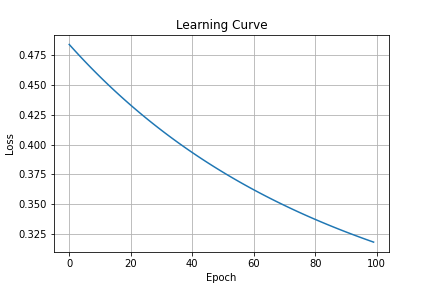
\includegraphics[width=0.8\textwidth]{Q1.png}
\caption{Loss vs Epoch}\label{fig:Q1}
\end{figure}
\begin{minipage}{0.3\textwidth}
    Training Loss = 0.32
\end{minipage}
\begin{minipage}{0.3\textwidth}
    Validation Loss = 0.32
\end{minipage}
\begin{minipage}{0.3\textwidth}
    Validation Accuracy = 50\%
\end{minipage}

\pagebreak

\section{Q2}

The number of training epochs is increased to 500.

\begin{figure}[h]
\centering
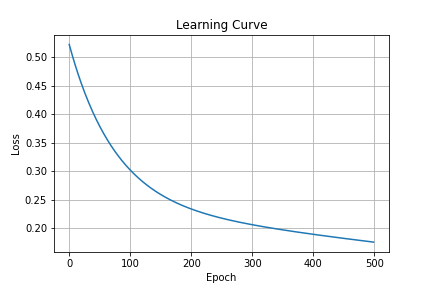
\includegraphics[width=0.8\textwidth]{Q2.png}
\caption{Loss vs Epoch}\label{fig:Q2}
\end{figure}
\begin{minipage}{0.3\textwidth}
    Training Loss = 0.17
\end{minipage}
\begin{minipage}{0.3\textwidth}
    Validation Loss = 0.18
\end{minipage}
\begin{minipage}{0.3\textwidth}
    Validation Accuracy = 93\%
\end{minipage}
\\
\\
With the increased number of epochs, the network fitted the training data better and all the evaluation metrics improved, including validation accuracy.

\pagebreak

\section{Q3}

Two addition fully connected layers are added to the network.

\begin{figure}[h]
\centering
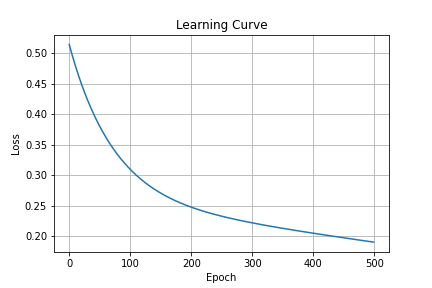
\includegraphics[width=0.8\textwidth]{Q3.png}
\caption{Loss vs Epoch}\label{fig:Q3}
\end{figure}
\begin{minipage}{0.3\textwidth}
    Training Loss = 0.19
\end{minipage}
\begin{minipage}{0.3\textwidth}
    Validation Loss = 0.20
\end{minipage}
\begin{minipage}{0.3\textwidth}
    Validation Accuracy = 80\%
\end{minipage}
\\
\\
Although adding a layer to the network increases the complexity of the decision boundaries, this network had lower accuracy and higher loss than the model in Figure~\ref{fig:Q2}. This situation may be attributed to fixed number of training epochs. The additional layers resulted the network to have more trainable parameters, hence it requires longer time to optimize them. 

\pagebreak

\section{Q4}

The learning rate is increased to $0.01$. 

\begin{figure}[h]
\centering
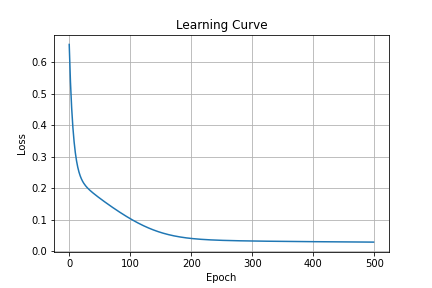
\includegraphics[width=0.8\textwidth]{Q4.png}
\caption{Loss vs Epoch}\label{fig:Q4}
\end{figure}
\begin{minipage}{0.3\textwidth}
    Training Loss = 0.02
\end{minipage}
\begin{minipage}{0.3\textwidth}
    Validation Loss = 0.02
\end{minipage}
\begin{minipage}{0.3\textwidth}
    Validation Accuracy = 98\%
\end{minipage}
\\
\\
With fixed number of training epochs, the network was able to achieve lower loss and higher validation accuracy. Since the networks weights are updated with larger steps in every iteration of backpropagation. Unlike what is observed in Figure~\ref{fig:Q2} and~\ref{fig:Q3}, the training loss stabilized at iteration 200 and it approaches at a lower number, namely 0.02.  

\pagebreak

\section{Q5}

A dropout layer with probability 0.5 is added to the network.

\begin{figure}[h]
\centering
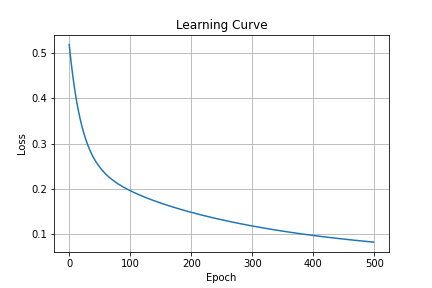
\includegraphics[width=0.8\textwidth]{Q5.png}
\caption{Loss vs Epoch}\label{fig:Q5}
\end{figure}
\begin{minipage}{0.3\textwidth}
    Training Loss = 0.08
\end{minipage}
\begin{minipage}{0.3\textwidth}
    Validation Loss = 0.08
\end{minipage}
\begin{minipage}{0.3\textwidth}
    Validation Accuracy = 96\%
\end{minipage}
\\
\\
Dropout layers are utilized to prevent the network from overfitting to the training data. When compared to the Figure~\ref{fig:Q4}, it can be observed that the both training and validation losses are higher, and validation accuracy decreased. 
\pagebreak

\section{Q6}

Momentum is added to the optimizer. 

\begin{figure}[h]
\centering
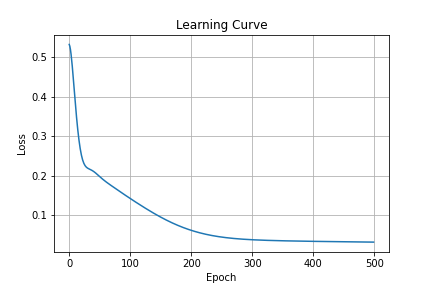
\includegraphics[width=0.8\textwidth]{Q6.png}
\caption{Loss vs Epoch}\label{fig:Q6}
\end{figure}
\begin{minipage}{0.3\textwidth}
    Training Loss = 0.03
\end{minipage}
\begin{minipage}{0.3\textwidth}
    Validation Loss = 0.02
\end{minipage}
\begin{minipage}{0.3\textwidth}
    Validation Accuracy = 97\%
\end{minipage}
\\
\\
The momentum provides a weighted sum of previous update terms to the network parameters, hence it provides a more stable convergence to the optimal point. It is possible to observe that momentum resulted the network to reach a training loss of 0.1 around $150^{th}$ epoch, whereas it was achieved in $400^{th}$ epoch in Figure~\ref{fig:Q5}

\pagebreak

\section{Appendix}

The code and results given in this section is shared 
\href{https://github.com/kutay-ugurlu/Pattern-Recognition/tree/master/HW6}{@\faGithubSquare}

    \begin{tcolorbox}[breakable, size=fbox, boxrule=1pt, pad at break*=1mm,colback=cellbackground, colframe=cellborder]
\prompt{In}{incolor}{ }{\boxspacing}
\begin{Verbatim}[commandchars=\\\{\}]
\PY{k+kn}{import} \PY{n+nn}{torch}
\PY{k+kn}{import} \PY{n+nn}{numpy} \PY{k}{as} \PY{n+nn}{np}
\PY{k+kn}{from} \PY{n+nn}{sklearn}\PY{n+nn}{.}\PY{n+nn}{datasets} \PY{k+kn}{import} \PY{n}{make\PYZus{}blobs}
\PY{k+kn}{import} \PY{n+nn}{matplotlib}\PY{n+nn}{.}\PY{n+nn}{pyplot} \PY{k}{as} \PY{n+nn}{plt}
\PY{k+kn}{import} \PY{n+nn}{json} 
\end{Verbatim}
\end{tcolorbox}

    \begin{tcolorbox}[breakable, size=fbox, boxrule=1pt, pad at break*=1mm,colback=cellbackground, colframe=cellborder]
\prompt{In}{incolor}{ }{\boxspacing}
\begin{Verbatim}[commandchars=\\\{\}]
\PY{k+kn}{from} \PY{n+nn}{google}\PY{n+nn}{.}\PY{n+nn}{colab} \PY{k+kn}{import} \PY{n}{drive}
\PY{n}{drive}\PY{o}{.}\PY{n}{mount}\PY{p}{(}\PY{l+s+s1}{\PYZsq{}}\PY{l+s+s1}{/content/drive}\PY{l+s+s1}{\PYZsq{}}\PY{p}{)}
\end{Verbatim}
\end{tcolorbox}

    \begin{tcolorbox}[breakable, size=fbox, boxrule=1pt, pad at break*=1mm,colback=cellbackground, colframe=cellborder]
\prompt{In}{incolor}{ }{\boxspacing}
\begin{Verbatim}[commandchars=\\\{\}]
\PY{c+c1}{\PYZsh{}DEFINE YOUR DEVICE}
\PY{n}{device} \PY{o}{=} \PY{n}{torch}\PY{o}{.}\PY{n}{device}\PY{p}{(}\PY{l+s+s1}{\PYZsq{}}\PY{l+s+s1}{cuda:0}\PY{l+s+s1}{\PYZsq{}} \PY{k}{if} \PY{n}{torch}\PY{o}{.}\PY{n}{cuda}\PY{o}{.}\PY{n}{is\PYZus{}available}\PY{p}{(}\PY{p}{)} \PY{k}{else} \PY{l+s+s1}{\PYZsq{}}\PY{l+s+s1}{cpu}\PY{l+s+s1}{\PYZsq{}}\PY{p}{)}

\PY{n+nb}{print}\PY{p}{(}\PY{n}{device}\PY{p}{)} \PY{c+c1}{\PYZsh{}if cpu, go Runtime\PYZhy{}\PYZgt{} Change runtime type\PYZhy{}\PYZgt{} Hardware accelerator GPU \PYZhy{}\PYZgt{} Save \PYZhy{}\PYZgt{} Redo previous steps}
\end{Verbatim}
\end{tcolorbox}

    \begin{tcolorbox}[breakable, size=fbox, boxrule=1pt, pad at break*=1mm,colback=cellbackground, colframe=cellborder]
\prompt{In}{incolor}{ }{\boxspacing}
\begin{Verbatim}[commandchars=\\\{\}]
\PY{c+c1}{\PYZsh{}CREATE A RANDOM DATASET}
\PY{n}{centers} \PY{o}{=} \PY{p}{[}\PY{p}{[}\PY{l+m+mi}{1}\PY{p}{,} \PY{l+m+mi}{1}\PY{p}{]}\PY{p}{,} \PY{p}{[}\PY{l+m+mi}{1}\PY{p}{,} \PY{o}{\PYZhy{}}\PY{l+m+mi}{1}\PY{p}{]}\PY{p}{,} \PY{p}{[}\PY{o}{\PYZhy{}}\PY{l+m+mi}{1}\PY{p}{,} \PY{o}{\PYZhy{}}\PY{l+m+mi}{1}\PY{p}{]}\PY{p}{,} \PY{p}{[}\PY{o}{\PYZhy{}}\PY{l+m+mi}{1}\PY{p}{,} \PY{l+m+mi}{1}\PY{p}{]}\PY{p}{]} \PY{c+c1}{\PYZsh{}center of each class}
\PY{n}{cluster\PYZus{}std}\PY{o}{=}\PY{l+m+mf}{0.4} \PY{c+c1}{\PYZsh{}standard deviation of random gaussian samples}

\PY{n}{x\PYZus{}train}\PY{p}{,} \PY{n}{y\PYZus{}train} \PY{o}{=} \PY{n}{make\PYZus{}blobs}\PY{p}{(}\PY{n}{n\PYZus{}samples}\PY{o}{=}\PY{l+m+mi}{1000}\PY{p}{,} \PY{n}{centers}\PY{o}{=}\PY{n}{centers}\PY{p}{,} \PY{n}{n\PYZus{}features}\PY{o}{=}\PY{l+m+mi}{2}\PY{p}{,} \PY{n}{cluster\PYZus{}std}\PY{o}{=}\PY{n}{cluster\PYZus{}std}\PY{p}{,} \PY{n}{shuffle}\PY{o}{=}\PY{k+kc}{True}\PY{p}{)}
\PY{n}{y\PYZus{}train}\PY{p}{[}\PY{n}{y\PYZus{}train}\PY{o}{==}\PY{l+m+mi}{2}\PY{p}{]} \PY{o}{=} \PY{l+m+mi}{0} \PY{c+c1}{\PYZsh{}make this an xor problem}
\PY{n}{y\PYZus{}train}\PY{p}{[}\PY{n}{y\PYZus{}train}\PY{o}{==}\PY{l+m+mi}{3}\PY{p}{]} \PY{o}{=} \PY{l+m+mi}{1} \PY{c+c1}{\PYZsh{}make this an xor problem}
\PY{n}{x\PYZus{}train} \PY{o}{=} \PY{n}{torch}\PY{o}{.}\PY{n}{FloatTensor}\PY{p}{(}\PY{n}{x\PYZus{}train}\PY{p}{)}
\PY{n}{y\PYZus{}train} \PY{o}{=} \PY{n}{torch}\PY{o}{.}\PY{n}{FloatTensor}\PY{p}{(}\PY{n}{y\PYZus{}train}\PY{p}{)}

\PY{n}{x\PYZus{}val}\PY{p}{,} \PY{n}{y\PYZus{}val} \PY{o}{=} \PY{n}{make\PYZus{}blobs}\PY{p}{(}\PY{n}{n\PYZus{}samples}\PY{o}{=}\PY{l+m+mi}{100}\PY{p}{,} \PY{n}{centers}\PY{o}{=}\PY{n}{centers}\PY{p}{,} \PY{n}{n\PYZus{}features}\PY{o}{=}\PY{l+m+mi}{2}\PY{p}{,} \PY{n}{cluster\PYZus{}std}\PY{o}{=}\PY{n}{cluster\PYZus{}std}\PY{p}{,} \PY{n}{shuffle}\PY{o}{=}\PY{k+kc}{True}\PY{p}{)}
\PY{n}{y\PYZus{}val}\PY{p}{[}\PY{n}{y\PYZus{}val}\PY{o}{==}\PY{l+m+mi}{2}\PY{p}{]} \PY{o}{=} \PY{l+m+mi}{0} \PY{c+c1}{\PYZsh{}make this an xor problem}
\PY{n}{y\PYZus{}val}\PY{p}{[}\PY{n}{y\PYZus{}val}\PY{o}{==}\PY{l+m+mi}{3}\PY{p}{]} \PY{o}{=} \PY{l+m+mi}{1} \PY{c+c1}{\PYZsh{}make this an xor problem}
\PY{n}{x\PYZus{}val} \PY{o}{=} \PY{n}{torch}\PY{o}{.}\PY{n}{FloatTensor}\PY{p}{(}\PY{n}{x\PYZus{}val}\PY{p}{)}
\PY{n}{y\PYZus{}val} \PY{o}{=} \PY{n}{torch}\PY{o}{.}\PY{n}{FloatTensor}\PY{p}{(}\PY{n}{y\PYZus{}val}\PY{p}{)}
\end{Verbatim}
\end{tcolorbox}

    \begin{tcolorbox}[breakable, size=fbox, boxrule=1pt, pad at break*=1mm,colback=cellbackground, colframe=cellborder]
\prompt{In}{incolor}{ }{\boxspacing}
\begin{Verbatim}[commandchars=\\\{\}]
\PY{c+c1}{\PYZsh{}CHECK THE BLOBS ON XY PLOT}
\PY{n}{plt}\PY{o}{.}\PY{n}{scatter}\PY{p}{(}\PY{n}{x\PYZus{}train}\PY{p}{[}\PY{n}{y\PYZus{}train}\PY{o}{==}\PY{l+m+mi}{0}\PY{p}{,}\PY{l+m+mi}{0}\PY{p}{]}\PY{p}{,}\PY{n}{x\PYZus{}train}\PY{p}{[}\PY{n}{y\PYZus{}train}\PY{o}{==}\PY{l+m+mi}{0}\PY{p}{,}\PY{l+m+mi}{1}\PY{p}{]}\PY{p}{,}\PY{n}{marker}\PY{o}{=}\PY{l+s+s1}{\PYZsq{}}\PY{l+s+s1}{o}\PY{l+s+s1}{\PYZsq{}}\PY{p}{,}\PY{n}{color}\PY{o}{=}\PY{l+s+s1}{\PYZsq{}}\PY{l+s+s1}{blue}\PY{l+s+s1}{\PYZsq{}}\PY{p}{)}
\PY{n}{plt}\PY{o}{.}\PY{n}{scatter}\PY{p}{(}\PY{n}{x\PYZus{}train}\PY{p}{[}\PY{n}{y\PYZus{}train}\PY{o}{==}\PY{l+m+mi}{1}\PY{p}{,}\PY{l+m+mi}{0}\PY{p}{]}\PY{p}{,}\PY{n}{x\PYZus{}train}\PY{p}{[}\PY{n}{y\PYZus{}train}\PY{o}{==}\PY{l+m+mi}{1}\PY{p}{,}\PY{l+m+mi}{1}\PY{p}{]}\PY{p}{,}\PY{n}{marker}\PY{o}{=}\PY{l+s+s1}{\PYZsq{}}\PY{l+s+s1}{o}\PY{l+s+s1}{\PYZsq{}}\PY{p}{,}\PY{n}{color}\PY{o}{=}\PY{l+s+s1}{\PYZsq{}}\PY{l+s+s1}{red}\PY{l+s+s1}{\PYZsq{}}\PY{p}{)}
\PY{n}{plt}\PY{o}{.}\PY{n}{savefig}\PY{p}{(}\PY{l+s+s1}{\PYZsq{}}\PY{l+s+s1}{/content/drive/MyDrive/583\PYZus{}HW6/dataset.png}\PY{l+s+s1}{\PYZsq{}}\PY{p}{)}
\end{Verbatim}
\end{tcolorbox}

    MODELS

    \begin{tcolorbox}[breakable, size=fbox, boxrule=1pt, pad at break*=1mm,colback=cellbackground, colframe=cellborder]
\prompt{In}{incolor}{ }{\boxspacing}
\begin{Verbatim}[commandchars=\\\{\}]
\PY{c+c1}{\PYZsh{}DEFINE NEURAL NETWORK MODEL}
\PY{k}{class} \PY{n+nc}{FullyConnected}\PY{p}{(}\PY{n}{torch}\PY{o}{.}\PY{n}{nn}\PY{o}{.}\PY{n}{Module}\PY{p}{)}\PY{p}{:}
  \PY{k}{def} \PY{n+nf+fm}{\PYZus{}\PYZus{}init\PYZus{}\PYZus{}}\PY{p}{(}\PY{n+nb+bp}{self}\PY{p}{,} \PY{n}{input\PYZus{}size}\PY{p}{,} \PY{n}{hidden\PYZus{}size}\PY{p}{,} \PY{n}{num\PYZus{}classes}\PY{p}{)}\PY{p}{:}
    \PY{n+nb}{super}\PY{p}{(}\PY{n}{FullyConnected}\PY{p}{,} \PY{n+nb+bp}{self}\PY{p}{)}\PY{o}{.}\PY{n+nf+fm}{\PYZus{}\PYZus{}init\PYZus{}\PYZus{}}\PY{p}{(}\PY{p}{)}
    \PY{n+nb+bp}{self}\PY{o}{.}\PY{n}{input\PYZus{}size} \PY{o}{=} \PY{n}{input\PYZus{}size}
    \PY{n+nb+bp}{self}\PY{o}{.}\PY{n}{hidden\PYZus{}size}  \PY{o}{=} \PY{n}{hidden\PYZus{}size}
    \PY{n+nb+bp}{self}\PY{o}{.}\PY{n}{fc1} \PY{o}{=} \PY{n}{torch}\PY{o}{.}\PY{n}{nn}\PY{o}{.}\PY{n}{Linear}\PY{p}{(}\PY{n+nb+bp}{self}\PY{o}{.}\PY{n}{input\PYZus{}size}\PY{p}{,} \PY{n+nb+bp}{self}\PY{o}{.}\PY{n}{hidden\PYZus{}size}\PY{p}{)}  
    \PY{n+nb+bp}{self}\PY{o}{.}\PY{n}{fc2} \PY{o}{=} \PY{n}{torch}\PY{o}{.}\PY{n}{nn}\PY{o}{.}\PY{n}{Linear}\PY{p}{(}\PY{n+nb+bp}{self}\PY{o}{.}\PY{n}{hidden\PYZus{}size}\PY{p}{,} \PY{n}{num\PYZus{}classes}\PY{p}{)}
    \PY{n+nb+bp}{self}\PY{o}{.}\PY{n}{relu} \PY{o}{=} \PY{n}{torch}\PY{o}{.}\PY{n}{nn}\PY{o}{.}\PY{n}{ReLU}\PY{p}{(}\PY{p}{)}
    \PY{n+nb+bp}{self}\PY{o}{.}\PY{n}{sigmoid} \PY{o}{=} \PY{n}{torch}\PY{o}{.}\PY{n}{nn}\PY{o}{.}\PY{n}{Sigmoid}\PY{p}{(}\PY{p}{)}
  \PY{k}{def} \PY{n+nf}{forward}\PY{p}{(}\PY{n+nb+bp}{self}\PY{p}{,} \PY{n}{x}\PY{p}{)}\PY{p}{:}
    \PY{n}{hidden} \PY{o}{=} \PY{n+nb+bp}{self}\PY{o}{.}\PY{n}{fc1}\PY{p}{(}\PY{n}{x}\PY{p}{)}
    \PY{n}{relu} \PY{o}{=} \PY{n+nb+bp}{self}\PY{o}{.}\PY{n}{relu}\PY{p}{(}\PY{n}{hidden}\PY{p}{)}
    \PY{n}{output} \PY{o}{=} \PY{n+nb+bp}{self}\PY{o}{.}\PY{n}{fc2}\PY{p}{(}\PY{n}{relu}\PY{p}{)}
    \PY{k}{return} \PY{n}{output}
\PY{k}{class} \PY{n+nc}{FullyConnectedModified}\PY{p}{(}\PY{n}{torch}\PY{o}{.}\PY{n}{nn}\PY{o}{.}\PY{n}{Module}\PY{p}{)}\PY{p}{:}
  \PY{k}{def} \PY{n+nf+fm}{\PYZus{}\PYZus{}init\PYZus{}\PYZus{}}\PY{p}{(}\PY{n+nb+bp}{self}\PY{p}{,} \PY{n}{input\PYZus{}size}\PY{p}{,} \PY{n}{hidden\PYZus{}size}\PY{p}{,} \PY{n}{num\PYZus{}classes}\PY{p}{)}\PY{p}{:}
    \PY{n+nb}{super}\PY{p}{(}\PY{n}{FullyConnectedModified}\PY{p}{,} \PY{n+nb+bp}{self}\PY{p}{)}\PY{o}{.}\PY{n+nf+fm}{\PYZus{}\PYZus{}init\PYZus{}\PYZus{}}\PY{p}{(}\PY{p}{)}
    \PY{n+nb+bp}{self}\PY{o}{.}\PY{n}{input\PYZus{}size} \PY{o}{=} \PY{n}{input\PYZus{}size}
    \PY{n+nb+bp}{self}\PY{o}{.}\PY{n}{hidden\PYZus{}size}  \PY{o}{=} \PY{n}{hidden\PYZus{}size}
    \PY{n+nb+bp}{self}\PY{o}{.}\PY{n}{fc1} \PY{o}{=} \PY{n}{torch}\PY{o}{.}\PY{n}{nn}\PY{o}{.}\PY{n}{Linear}\PY{p}{(}\PY{n+nb+bp}{self}\PY{o}{.}\PY{n}{input\PYZus{}size}\PY{p}{,} \PY{n+nb+bp}{self}\PY{o}{.}\PY{n}{hidden\PYZus{}size}\PY{p}{)}  
    \PY{n+nb+bp}{self}\PY{o}{.}\PY{n}{fc2} \PY{o}{=} \PY{n}{torch}\PY{o}{.}\PY{n}{nn}\PY{o}{.}\PY{n}{Linear}\PY{p}{(}\PY{n+nb+bp}{self}\PY{o}{.}\PY{n}{hidden\PYZus{}size}\PY{p}{,} \PY{l+m+mi}{2}\PY{o}{*}\PY{n+nb+bp}{self}\PY{o}{.}\PY{n}{hidden\PYZus{}size}\PY{p}{)}
    \PY{n+nb+bp}{self}\PY{o}{.}\PY{n}{fc3} \PY{o}{=} \PY{n}{torch}\PY{o}{.}\PY{n}{nn}\PY{o}{.}\PY{n}{Linear}\PY{p}{(}\PY{l+m+mi}{2}\PY{o}{*}\PY{n+nb+bp}{self}\PY{o}{.}\PY{n}{hidden\PYZus{}size}\PY{p}{,} \PY{l+m+mi}{4}\PY{o}{*}\PY{n+nb+bp}{self}\PY{o}{.}\PY{n}{hidden\PYZus{}size}\PY{p}{)}
    \PY{n+nb+bp}{self}\PY{o}{.}\PY{n}{fc4} \PY{o}{=} \PY{n}{torch}\PY{o}{.}\PY{n}{nn}\PY{o}{.}\PY{n}{Linear}\PY{p}{(}\PY{l+m+mi}{4}\PY{o}{*}\PY{n+nb+bp}{self}\PY{o}{.}\PY{n}{hidden\PYZus{}size}\PY{p}{,} \PY{n}{num\PYZus{}classes}\PY{p}{)}
    \PY{n+nb+bp}{self}\PY{o}{.}\PY{n}{relu} \PY{o}{=} \PY{n}{torch}\PY{o}{.}\PY{n}{nn}\PY{o}{.}\PY{n}{ReLU}\PY{p}{(}\PY{p}{)}
    \PY{n+nb+bp}{self}\PY{o}{.}\PY{n}{sigmoid} \PY{o}{=} \PY{n}{torch}\PY{o}{.}\PY{n}{nn}\PY{o}{.}\PY{n}{Sigmoid}\PY{p}{(}\PY{p}{)}
  \PY{k}{def} \PY{n+nf}{forward}\PY{p}{(}\PY{n+nb+bp}{self}\PY{p}{,} \PY{n}{x}\PY{p}{)}\PY{p}{:}
    \PY{n}{hidden1} \PY{o}{=} \PY{n+nb+bp}{self}\PY{o}{.}\PY{n}{fc1}\PY{p}{(}\PY{n}{x}\PY{p}{)}
    \PY{n}{relu} \PY{o}{=} \PY{n+nb+bp}{self}\PY{o}{.}\PY{n}{relu}\PY{p}{(}\PY{n}{hidden1}\PY{p}{)}
    \PY{n}{hidden2} \PY{o}{=} \PY{n+nb+bp}{self}\PY{o}{.}\PY{n}{fc2}\PY{p}{(}\PY{n}{relu}\PY{p}{)}
    \PY{n}{relu2} \PY{o}{=} \PY{n+nb+bp}{self}\PY{o}{.}\PY{n}{relu}\PY{p}{(}\PY{n}{hidden2}\PY{p}{)}
    \PY{n}{hidden3} \PY{o}{=} \PY{n+nb+bp}{self}\PY{o}{.}\PY{n}{fc3}\PY{p}{(}\PY{n}{relu2}\PY{p}{)}
    \PY{n}{relu3} \PY{o}{=} \PY{n+nb+bp}{self}\PY{o}{.}\PY{n}{relu}\PY{p}{(}\PY{n}{hidden3}\PY{p}{)}
    \PY{n}{output} \PY{o}{=} \PY{n+nb+bp}{self}\PY{o}{.}\PY{n}{fc4}\PY{p}{(}\PY{n}{relu3}\PY{p}{)}
    \PY{k}{return} \PY{n}{output}
\PY{k}{class} \PY{n+nc}{FullyConnectedQ5}\PY{p}{(}\PY{n}{torch}\PY{o}{.}\PY{n}{nn}\PY{o}{.}\PY{n}{Module}\PY{p}{)}\PY{p}{:}
  \PY{k}{def} \PY{n+nf+fm}{\PYZus{}\PYZus{}init\PYZus{}\PYZus{}}\PY{p}{(}\PY{n+nb+bp}{self}\PY{p}{,} \PY{n}{input\PYZus{}size}\PY{p}{,} \PY{n}{hidden\PYZus{}size}\PY{p}{,} \PY{n}{num\PYZus{}classes}\PY{p}{)}\PY{p}{:}
    \PY{n+nb}{super}\PY{p}{(}\PY{n}{FullyConnectedQ5}\PY{p}{,} \PY{n+nb+bp}{self}\PY{p}{)}\PY{o}{.}\PY{n+nf+fm}{\PYZus{}\PYZus{}init\PYZus{}\PYZus{}}\PY{p}{(}\PY{p}{)}
    \PY{n+nb+bp}{self}\PY{o}{.}\PY{n}{input\PYZus{}size} \PY{o}{=} \PY{n}{input\PYZus{}size}
    \PY{n+nb+bp}{self}\PY{o}{.}\PY{n}{hidden\PYZus{}size}  \PY{o}{=} \PY{n}{hidden\PYZus{}size}
    \PY{n+nb+bp}{self}\PY{o}{.}\PY{n}{fc1} \PY{o}{=} \PY{n}{torch}\PY{o}{.}\PY{n}{nn}\PY{o}{.}\PY{n}{Linear}\PY{p}{(}\PY{n+nb+bp}{self}\PY{o}{.}\PY{n}{input\PYZus{}size}\PY{p}{,} \PY{n+nb+bp}{self}\PY{o}{.}\PY{n}{hidden\PYZus{}size}\PY{p}{)}  
    \PY{n+nb+bp}{self}\PY{o}{.}\PY{n}{fc2} \PY{o}{=} \PY{n}{torch}\PY{o}{.}\PY{n}{nn}\PY{o}{.}\PY{n}{Linear}\PY{p}{(}\PY{n+nb+bp}{self}\PY{o}{.}\PY{n}{hidden\PYZus{}size}\PY{p}{,} \PY{n}{num\PYZus{}classes}\PY{p}{)}
    \PY{n+nb+bp}{self}\PY{o}{.}\PY{n}{relu} \PY{o}{=} \PY{n}{torch}\PY{o}{.}\PY{n}{nn}\PY{o}{.}\PY{n}{ReLU}\PY{p}{(}\PY{p}{)}
    \PY{n+nb+bp}{self}\PY{o}{.}\PY{n}{dropout} \PY{o}{=} \PY{n}{torch}\PY{o}{.}\PY{n}{nn}\PY{o}{.}\PY{n}{Dropout}\PY{p}{(}\PY{l+m+mf}{0.5}\PY{p}{)}
    \PY{n+nb+bp}{self}\PY{o}{.}\PY{n}{sigmoid} \PY{o}{=} \PY{n}{torch}\PY{o}{.}\PY{n}{nn}\PY{o}{.}\PY{n}{Sigmoid}\PY{p}{(}\PY{p}{)}
  \PY{k}{def} \PY{n+nf}{forward}\PY{p}{(}\PY{n+nb+bp}{self}\PY{p}{,} \PY{n}{x}\PY{p}{)}\PY{p}{:}
    \PY{n}{hidden} \PY{o}{=} \PY{n+nb+bp}{self}\PY{o}{.}\PY{n}{fc1}\PY{p}{(}\PY{n}{x}\PY{p}{)}
    \PY{n}{relu} \PY{o}{=} \PY{n+nb+bp}{self}\PY{o}{.}\PY{n}{relu}\PY{p}{(}\PY{n}{hidden}\PY{p}{)}
    \PY{n}{dropout} \PY{o}{=} \PY{n+nb+bp}{self}\PY{o}{.}\PY{n}{dropout}\PY{p}{(}\PY{n}{relu}\PY{p}{)}
    \PY{n}{output} \PY{o}{=} \PY{n+nb+bp}{self}\PY{o}{.}\PY{n}{fc2}\PY{p}{(}\PY{n}{relu}\PY{p}{)}
    \PY{k}{return} \PY{n}{output}
\end{Verbatim}
\end{tcolorbox}

    \begin{tcolorbox}[breakable, size=fbox, boxrule=1pt, pad at break*=1mm,colback=cellbackground, colframe=cellborder]
\prompt{In}{incolor}{ }{\boxspacing}
\begin{Verbatim}[commandchars=\\\{\}]
\PY{n}{output\PYZus{}path} \PY{o}{=} \PY{l+s+s2}{\PYZdq{}}\PY{l+s+s2}{/content/drive/MyDrive/583\PYZus{}HW6}\PY{l+s+s2}{\PYZdq{}}
\PY{k}{for} \PY{n}{question} \PY{o+ow}{in} \PY{p}{[}\PY{n+nb}{str}\PY{p}{(}\PY{n}{i}\PY{p}{)} \PY{k}{for} \PY{n}{i} \PY{o+ow}{in} \PY{n+nb}{range}\PY{p}{(}\PY{l+m+mi}{1}\PY{p}{,}\PY{l+m+mi}{7}\PY{p}{)}\PY{p}{]}\PY{p}{:}

  \PY{c+c1}{\PYZsh{}CREATE MODEL}
  \PY{n}{input\PYZus{}size} \PY{o}{=} \PY{l+m+mi}{2}
  \PY{n}{hidden\PYZus{}size} \PY{o}{=} \PY{l+m+mi}{64}
  \PY{n}{num\PYZus{}classes} \PY{o}{=} \PY{l+m+mi}{1}

  \PY{n}{model} \PY{o}{=} \PY{n}{FullyConnected}\PY{p}{(}\PY{n}{input\PYZus{}size}\PY{p}{,} \PY{n}{hidden\PYZus{}size}\PY{p}{,} \PY{n}{num\PYZus{}classes}\PY{p}{)} \PY{k}{if} \PY{n}{question} \PY{o}{==} \PY{l+s+s1}{\PYZsq{}}\PY{l+s+s1}{5}\PY{l+s+s1}{\PYZsq{}} \PY{k}{else} \PY{p}{(}\PY{n}{FullyConnectedModified}\PY{p}{(}\PY{n}{input\PYZus{}size}\PY{p}{,} \PY{n}{hidden\PYZus{}size}\PY{p}{,} \PY{n}{num\PYZus{}classes}\PY{p}{)} \PY{k}{if} \PY{n}{question} \PY{o}{==} \PY{l+s+s1}{\PYZsq{}}\PY{l+s+s1}{3}\PY{l+s+s1}{\PYZsq{}} \PY{o+ow}{or} \PY{n}{question} \PY{o}{==} \PY{l+s+s1}{\PYZsq{}}\PY{l+s+s1}{4}\PY{l+s+s1}{\PYZsq{}} \PY{k}{else} \PY{n}{FullyConnectedModified}\PY{p}{(}\PY{n}{input\PYZus{}size}\PY{p}{,} \PY{n}{hidden\PYZus{}size}\PY{p}{,} \PY{n}{num\PYZus{}classes}\PY{p}{)}\PY{p}{)}

  \PY{n}{model}\PY{o}{.}\PY{n}{to}\PY{p}{(}\PY{n}{device}\PY{p}{)}

  \PY{c+c1}{\PYZsh{}DEFINE LOSS FUNCTION AND OPTIMIZER}
  \PY{n}{learning\PYZus{}rate} \PY{o}{=} \PY{l+m+mf}{0.01} \PY{k}{if} \PY{n}{question} \PY{o}{==} \PY{l+s+s1}{\PYZsq{}}\PY{l+s+s1}{4}\PY{l+s+s1}{\PYZsq{}} \PY{k}{else} \PY{l+m+mf}{0.001}
  \PY{n}{momentum} \PY{o}{=} \PY{l+m+mf}{0.9} \PY{k}{if} \PY{n}{question} \PY{o}{==} \PY{l+s+s1}{\PYZsq{}}\PY{l+s+s1}{6}\PY{l+s+s1}{\PYZsq{}} \PY{k}{else} \PY{l+m+mi}{0}

  \PY{n}{loss\PYZus{}fun} \PY{o}{=} \PY{n}{torch}\PY{o}{.}\PY{n}{nn}\PY{o}{.}\PY{n}{MSELoss}\PY{p}{(}\PY{p}{)}
  \PY{n}{optimizer} \PY{o}{=} \PY{n}{torch}\PY{o}{.}\PY{n}{optim}\PY{o}{.}\PY{n}{SGD}\PY{p}{(}\PY{n}{model}\PY{o}{.}\PY{n}{parameters}\PY{p}{(}\PY{p}{)}\PY{p}{,} \PY{n}{lr} \PY{o}{=} \PY{n}{learning\PYZus{}rate}\PY{p}{,} \PY{n}{momentum} \PY{o}{=} \PY{n}{momentum}\PY{p}{)}

  \PY{n}{model}\PY{o}{.}\PY{n}{train}\PY{p}{(}\PY{p}{)}
  \PY{n}{epoch} \PY{o}{=} \PY{l+m+mi}{100} \PY{k}{if} \PY{n}{question} \PY{o}{==} \PY{l+s+s1}{\PYZsq{}}\PY{l+s+s1}{1}\PY{l+s+s1}{\PYZsq{}} \PY{k}{else} \PY{l+m+mi}{500}
  \PY{n}{x\PYZus{}train} \PY{o}{=} \PY{n}{x\PYZus{}train}\PY{o}{.}\PY{n}{to}\PY{p}{(}\PY{n}{device}\PY{p}{)}
  \PY{n}{y\PYZus{}train} \PY{o}{=} \PY{n}{y\PYZus{}train}\PY{o}{.}\PY{n}{to}\PY{p}{(}\PY{n}{device}\PY{p}{)}

  \PY{n}{loss\PYZus{}values} \PY{o}{=} \PY{n}{np}\PY{o}{.}\PY{n}{zeros}\PY{p}{(}\PY{n}{epoch}\PY{p}{)}

  \PY{c+c1}{\PYZsh{} TRAIN THE MODEL}
  \PY{k}{for} \PY{n}{i} \PY{o+ow}{in} \PY{n+nb}{range}\PY{p}{(}\PY{n}{epoch}\PY{p}{)}\PY{p}{:}
      \PY{n}{optimizer}\PY{o}{.}\PY{n}{zero\PYZus{}grad}\PY{p}{(}\PY{p}{)}    
      \PY{n}{y\PYZus{}pred} \PY{o}{=} \PY{n}{model}\PY{p}{(}\PY{n}{x\PYZus{}train}\PY{p}{)}    \PY{c+c1}{\PYZsh{} forward}
      \PY{c+c1}{\PYZsh{}reshape y\PYZus{}pred from (n\PYZus{}samples,1) to (n\PYZus{}samples), so y\PYZus{}pred and y\PYZus{}train have the same shape}
      \PY{n}{y\PYZus{}pred} \PY{o}{=} \PY{n}{y\PYZus{}pred}\PY{o}{.}\PY{n}{reshape}\PY{p}{(}\PY{n}{y\PYZus{}pred}\PY{o}{.}\PY{n}{shape}\PY{p}{[}\PY{l+m+mi}{0}\PY{p}{]}\PY{p}{)}
      \PY{n}{loss} \PY{o}{=} \PY{n}{loss\PYZus{}fun}\PY{p}{(}\PY{n}{y\PYZus{}pred}\PY{p}{,} \PY{n}{y\PYZus{}train}\PY{p}{)}
    
      \PY{n}{loss\PYZus{}values}\PY{p}{[}\PY{n}{i}\PY{p}{]} \PY{o}{=} \PY{n}{loss}\PY{o}{.}\PY{n}{item}\PY{p}{(}\PY{p}{)}
      \PY{n+nb}{print}\PY{p}{(}\PY{l+s+s1}{\PYZsq{}}\PY{l+s+s1}{Epoch }\PY{l+s+si}{\PYZob{}\PYZcb{}}\PY{l+s+s1}{: train loss: }\PY{l+s+si}{\PYZob{}\PYZcb{}}\PY{l+s+s1}{\PYZsq{}}\PY{o}{.}\PY{n}{format}\PY{p}{(}\PY{n}{i}\PY{p}{,} \PY{n}{loss}\PY{o}{.}\PY{n}{item}\PY{p}{(}\PY{p}{)}\PY{p}{)}\PY{p}{)}    
      \PY{n}{loss}\PY{o}{.}\PY{n}{backward}\PY{p}{(}\PY{p}{)} \PY{c+c1}{\PYZsh{}backward}
      \PY{n}{optimizer}\PY{o}{.}\PY{n}{step}\PY{p}{(}\PY{p}{)}  

  \PY{n}{training\PYZus{}loss} \PY{o}{=} \PY{n}{loss}\PY{o}{.}\PY{n}{item}\PY{p}{(}\PY{p}{)}

  \PY{c+c1}{\PYZsh{}PLOT THE LEARNING CURVE}
  \PY{n}{plt}\PY{o}{.}\PY{n}{figure}
  \PY{n}{plt}\PY{o}{.}\PY{n}{plot}\PY{p}{(}\PY{n}{loss\PYZus{}values}\PY{p}{)}
  \PY{n}{plt}\PY{o}{.}\PY{n}{title}\PY{p}{(}\PY{l+s+s1}{\PYZsq{}}\PY{l+s+s1}{Learning Curve}\PY{l+s+s1}{\PYZsq{}}\PY{p}{)}
  \PY{n}{plt}\PY{o}{.}\PY{n}{xlabel}\PY{p}{(}\PY{l+s+s1}{\PYZsq{}}\PY{l+s+s1}{Epoch}\PY{l+s+s1}{\PYZsq{}}\PY{p}{)}
  \PY{n}{plt}\PY{o}{.}\PY{n}{ylabel}\PY{p}{(}\PY{l+s+s1}{\PYZsq{}}\PY{l+s+s1}{Loss}\PY{l+s+s1}{\PYZsq{}}\PY{p}{)}
  \PY{n}{plt}\PY{o}{.}\PY{n}{grid}\PY{p}{(}\PY{l+s+s1}{\PYZsq{}}\PY{l+s+s1}{on}\PY{l+s+s1}{\PYZsq{}}\PY{p}{)}  

  \PY{n}{plt}\PY{o}{.}\PY{n}{savefig}\PY{p}{(}\PY{l+s+s1}{\PYZsq{}}\PY{l+s+s1}{/content/drive/MyDrive/583\PYZus{}HW6/Q}\PY{l+s+s1}{\PYZsq{}}\PY{o}{+}\PY{n}{question}\PY{o}{+}\PY{l+s+s1}{\PYZsq{}}\PY{l+s+s1}{.png}\PY{l+s+s1}{\PYZsq{}}\PY{p}{)}
  \PY{n}{plt}\PY{o}{.}\PY{n}{close}\PY{p}{(}\PY{l+s+s1}{\PYZsq{}}\PY{l+s+s1}{all}\PY{l+s+s1}{\PYZsq{}}\PY{p}{)}

  \PY{c+c1}{\PYZsh{}TEST THE MODEL}
  \PY{n}{model}\PY{o}{.}\PY{n}{eval}\PY{p}{(}\PY{p}{)}

  \PY{n}{x\PYZus{}val} \PY{o}{=} \PY{n}{x\PYZus{}val}\PY{o}{.}\PY{n}{to}\PY{p}{(}\PY{n}{device}\PY{p}{)}
  \PY{n}{y\PYZus{}val} \PY{o}{=} \PY{n}{y\PYZus{}val}\PY{o}{.}\PY{n}{to}\PY{p}{(}\PY{n}{device}\PY{p}{)}

  \PY{n}{y\PYZus{}pred} \PY{o}{=} \PY{n}{model}\PY{p}{(}\PY{n}{x\PYZus{}val}\PY{p}{)}
  \PY{c+c1}{\PYZsh{}reshape y\PYZus{}pred from (n\PYZus{}samples,1) to (n\PYZus{}samples), so y\PYZus{}pred and y\PYZus{}val have the same shape}
  \PY{n}{y\PYZus{}pred} \PY{o}{=} \PY{n}{y\PYZus{}pred}\PY{o}{.}\PY{n}{reshape}\PY{p}{(}\PY{n}{y\PYZus{}pred}\PY{o}{.}\PY{n}{shape}\PY{p}{[}\PY{l+m+mi}{0}\PY{p}{]}\PY{p}{)}
  \PY{n}{after\PYZus{}train} \PY{o}{=} \PY{n}{loss\PYZus{}fun}\PY{p}{(}\PY{n}{y\PYZus{}pred}\PY{p}{,} \PY{n}{y\PYZus{}val}\PY{p}{)} 
  \PY{n+nb}{print}\PY{p}{(}\PY{l+s+s1}{\PYZsq{}}\PY{l+s+s1}{Validation loss after Training}\PY{l+s+s1}{\PYZsq{}} \PY{p}{,} \PY{n}{after\PYZus{}train}\PY{o}{.}\PY{n}{item}\PY{p}{(}\PY{p}{)}\PY{p}{)}

  \PY{n}{correct}\PY{o}{=}\PY{l+m+mi}{0}
  \PY{n}{total}\PY{o}{=}\PY{l+m+mi}{0}
  \PY{k}{for} \PY{n}{i} \PY{o+ow}{in} \PY{n+nb}{range}\PY{p}{(}\PY{n}{y\PYZus{}pred}\PY{o}{.}\PY{n}{shape}\PY{p}{[}\PY{l+m+mi}{0}\PY{p}{]}\PY{p}{)}\PY{p}{:}
    \PY{k}{if} \PY{n}{y\PYZus{}val}\PY{p}{[}\PY{n}{i}\PY{p}{]}\PY{o}{==}\PY{n}{torch}\PY{o}{.}\PY{n}{round}\PY{p}{(}\PY{n}{y\PYZus{}pred}\PY{p}{[}\PY{n}{i}\PY{p}{]}\PY{p}{)}\PY{p}{:}
      \PY{n}{correct} \PY{o}{+}\PY{o}{=} \PY{l+m+mi}{1}
    \PY{n}{total} \PY{o}{+}\PY{o}{=}\PY{l+m+mi}{1}

  \PY{n}{val\PYZus{}acc} \PY{o}{=} \PY{p}{(}\PY{l+m+mi}{100}\PY{o}{*}\PY{n}{correct}\PY{p}{)}\PY{o}{/}\PY{o}{/}\PY{p}{(}\PY{n}{total}\PY{p}{)}
  \PY{n+nb}{print}\PY{p}{(}\PY{l+s+s1}{\PYZsq{}}\PY{l+s+s1}{Validation accuracy: }\PY{l+s+si}{\PYZpc{}.2f}\PY{l+s+si}{\PYZpc{}\PYZpc{}}\PY{l+s+s1}{\PYZsq{}} \PY{o}{\PYZpc{}}\PY{p}{(}\PY{p}{(}\PY{l+m+mi}{100}\PY{o}{*}\PY{n}{correct}\PY{p}{)}\PY{o}{/}\PY{o}{/}\PY{p}{(}\PY{n}{total}\PY{p}{)}\PY{p}{)}\PY{p}{)}  
  \PY{n}{val\PYZus{}acc}
  \PY{n}{result\PYZus{}dict} \PY{o}{=} \PY{p}{\PYZob{}}\PY{p}{\PYZcb{}}
  \PY{n}{result\PYZus{}dict}\PY{p}{[}\PY{l+s+s2}{\PYZdq{}}\PY{l+s+s2}{loss}\PY{l+s+s2}{\PYZdq{}}\PY{p}{]} \PY{o}{=} \PY{n}{after\PYZus{}train}\PY{o}{.}\PY{n}{item}\PY{p}{(}\PY{p}{)}
  \PY{n}{result\PYZus{}dict}\PY{p}{[}\PY{l+s+s2}{\PYZdq{}}\PY{l+s+s2}{acc}\PY{l+s+s2}{\PYZdq{}}\PY{p}{]} \PY{o}{=} \PY{n}{val\PYZus{}acc}
  \PY{n}{result\PYZus{}dict}\PY{p}{[}\PY{l+s+s2}{\PYZdq{}}\PY{l+s+s2}{trainingloss}\PY{l+s+s2}{\PYZdq{}}\PY{p}{]} \PY{o}{=} \PY{n}{training\PYZus{}loss}
  \PY{k}{with} \PY{n+nb}{open}\PY{p}{(}\PY{l+s+s1}{\PYZsq{}}\PY{l+s+s1}{/content/drive/MyDrive/583\PYZus{}HW6/result\PYZus{}dict\PYZus{}Q}\PY{l+s+s1}{\PYZsq{}} \PY{o}{+} \PY{n}{question} \PY{o}{+} \PY{l+s+s1}{\PYZsq{}}\PY{l+s+s1}{.json}\PY{l+s+s1}{\PYZsq{}}\PY{p}{,} \PY{l+s+s1}{\PYZsq{}}\PY{l+s+s1}{w}\PY{l+s+s1}{\PYZsq{}}\PY{p}{)} \PY{k}{as} \PY{n}{f}\PY{p}{:}
      \PY{n}{json}\PY{o}{.}\PY{n}{dump}\PY{p}{(}\PY{n}{result\PYZus{}dict}\PY{p}{,} \PY{n}{f}\PY{p}{)}
\end{Verbatim}
\end{tcolorbox}
\end{document}
